\chapter{Data Mining And Machine Learning}


    \textbf{Machine Learning:} develops system that learn from data and improve their performance without explicit programming. Model are automatically learned from data with minimal human intervention. The process is refined continuously based on experience and new information.\\
    \textbf{Data Mining:} analyzes large dataset to extract useful knowledge, helping organizations solve problems, predict trends, reduce risk, and discorver opportunities.
    If we really want to distinguish the two concepts, we could say that Machine Learning focuses more on how to obtain information, while Data Mining focuses more on what the information is used for.
    But in practice, the two terms are often used interchangeably.



\subsection{Bonferroni’s Principle}

A common data-mining problem is discovering unusual events hidden in massive datasets. However, even if the data is completely random, some events of interest will occur purely by chance. These occurrences are \textbf{bogus} and have no causal basis.  

The Bonferroni correction provides a statistically sound way to avoid most false positives. By calculating the expected number of random occurrences, we can judge whether apparent patterns are likely meaningful or just random noise.  


\subsection{Example: Detecting ``Evil-doers'' in Hotel Data}

Suppose there are believed to be some ``evil-doers,'' and we want to detect them. We assume that periodically, evil-doers gather at a hotel. The following assumptions define the problem size:
\begin{compactitemize}
    \item 1 billion potential people of interest.
    \item Each person visits a hotel 1 day out of 100.
    \item 100,000 hotels, each holding 100 people.
    \item Data covers 1000 days.
\end{compactitemize}

We look for people appearing at the same hotel on two different days. Suppose, however, that there really are no evil-doers, i.e., everyone behaves randomly: each person independently decides to visit a hotel with probability $0.01$ on a given day and chooses one of 100,000 hotels at random.

\textbf{Statistical calculation:}
\begin{compactitemize}
    \item Probability a person visits a hotel on any given day: $P(\text{visit per day}) = 0.01$
    \item Probability two people both visit a hotel on the same day: $0.01^2 = 0.0001$
    \item Probability they visit the same hotel on that day: $\frac{0.0001}{100,000} = 10^{-9}$
    \item Probability they meet at the same hotel on two different days: $(10^{-9})^2 = 10^{-18}$
    \item Number of possible pairs of people: $\binom{10^9}{2} \approx 5 \cdot 10^{17}$
    \item Number of possible pairs of days: $\binom{1000}{2} \approx 5 \cdot 10^5$
    \item Expected number of events that look like evil-doing: $5 \cdot 10^{17} \cdot 5 \cdot 10^5 \cdot 10^{-18} \approx 250,000$
\end{compactitemize}

Even though everyone behaves randomly, about 250,000 pairs appear to meet the ``evil-doer'' criterion. These pairs arise purely by chance due to the large dataset. 

Now, suppose there really are only 10 pairs of actual evil-doers. The police would need to investigate a quarter of a million other pairs to find the real ones. Besides intruding on the lives of half a million innocent people, the workload makes this approach practically infeasible. This example illustrates the importance of statistical corrections (like Bonferroni) to avoid being misled by spurious patterns in massive datasets.


\begin{figure}[H]
    \centering
    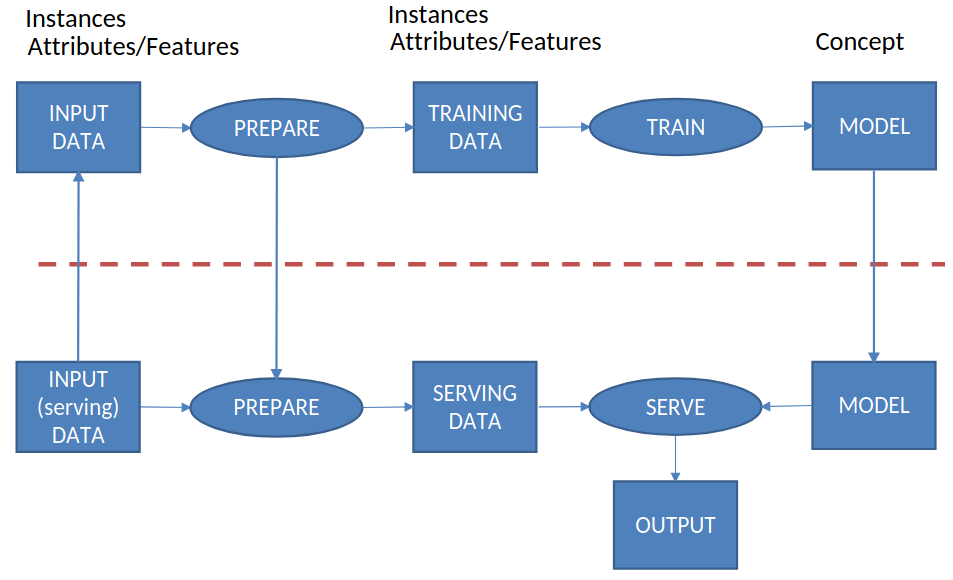
\includegraphics[width=0.7\textwidth]{images/ML_pipeline.png}
    \caption{The ML Pipeline}
    \label{fig:The ML Pipeline}
\end{figure}


    The image above illustrates the pipeline of an ML model used in industry. The part above the line also includes the test phase. The main point to note is the arrow from "INPUT (serving) DATA" back to "INPUT DATA." This arrow shows how the data generated while the model is in use becomes new training data for the model itself. Note that not all the generated data will be added to the training set, but only a small portion.


\section{Input: Concepts, Istance and Attributes}

    A model can be done various things, the principal are:
    \begin{compactitemize}
        \item \textbf{Classification:} Predicting a discrete class.
        \item \textbf{Numeric Prediction (Regression):} Predicting a numeric quantity.
        \item \textbf{Clustering:} Grouping a similar instance into clusters.
        \item \textbf{Data Reduction:} to replace a large set of data with a smaller set that contains much of the important information.
        \item \textbf{Association Learning:} detecting associations between features.
        \item \textbf{Similarity Matching:} identifying similar individuals based on data known about them.
        \item \textbf{Profiling:} characterizing the typical behavior of an inidvidual, group or population.
        \item \textbf{Link Prediction:} predicting connections between data items.
        \item \textbf{Casual Modeling:} to understand what events or actions actually influence others-
        \item \textbf{Embeddings:} semantic vector rappresentation of data, where data points (such as word, images, or categorical variables) are encoded as continuos vectors in a multi-dimesional space.
    \end{compactitemize}


\subsection{Unsupervised VS Supervised Learning}

    To distinguish between supervised and unsupervised learning, we can consider two similar questions:
    \begin{compactitemize}
        \item \textbf{Unsupervised:} Do our customers naturally fall into different groups?
        \item \textbf{Supervised:} Can we find groups of customers who have a particularly high likelihood of canceling their service soon after their contracts expire?
    \end{compactitemize}
    
    In the first question, there isn't a specific purpose or target for separating the groups. When there is no such target, the data mining problem is referred to as \textbf{unsupervised}.\\
    
    In the second question, the separation of the groups is based on a condition or purpose. This type of problem is referred to as \textbf{supervised}.


\subsection{Classification Learning}

Classification learning is a type of \textbf{supervised} learning. Example problems include weather data, contact lenses, irises, and labor negotiations.The model learns under the supervision provided by the actual outcomes of the training examples. Each outcome is called the \textbf{class} of the example.  

Success is measured on test data for which class labels are known.


\subsection{Numeric Prediction (Regression)}

Numeric prediction, also called \textbf{regression}, is a variant of classification learning where the “class” is numeric. This is also a \textbf{supervised} task. The model is provided with a target value and is trained to predict it. Success is measured on test data with known target values.


\subsection{Clustering}

Clustering involves finding groups of items that naturally fall together, e.g., discovering whether customers form natural segments.  Clustering is an \textbf{unsupervised} task: the class of each example is unknown. Success is often measured subjectively, based on how useful the result appears to a human user.



\subsection{Association Learning}

Association learning aims to discover patterns where multiple attributes occur together. Example problems include identifying which items are commonly purchased together.  

Differences from classification learning:  
\begin{compactitemize}
    \item Can predict any attribute’s value, not just the class.  
    \item Can predict more than one attribute at a time.  
    \item This generates far more association rules than classification rules, so \textbf{constraints} are necessary.  
    \item Constraints include minimum coverage (e.g., 80\% of the dataset) and minimum accuracy (e.g., 95\% accurate).  
\end{compactitemize}


\subsection{Issues in Flattening Data}

The process of flattening, called \textbf{denormalization}, involves joining multiple relations to create a single table.  

Problems:  
\begin{compactitemize}
    \item Denormalization may produce spurious regularities that reflect the database structure rather than meaningful patterns.  
    \item Example: ``supplier'' predicts ``supplier address.''  
\end{compactitemize}




\newpage
\section{Output: Knowledge Representation}

\subsection{Data Mining vs. Results Usage}

    There is an important distinction in data mining between:
    \begin{compactitemize}
        \item Mining data to find patterns and build models.
        \item Using the results of data mining
    \end{compactitemize}


\begin{figure}[H]
    \centering
    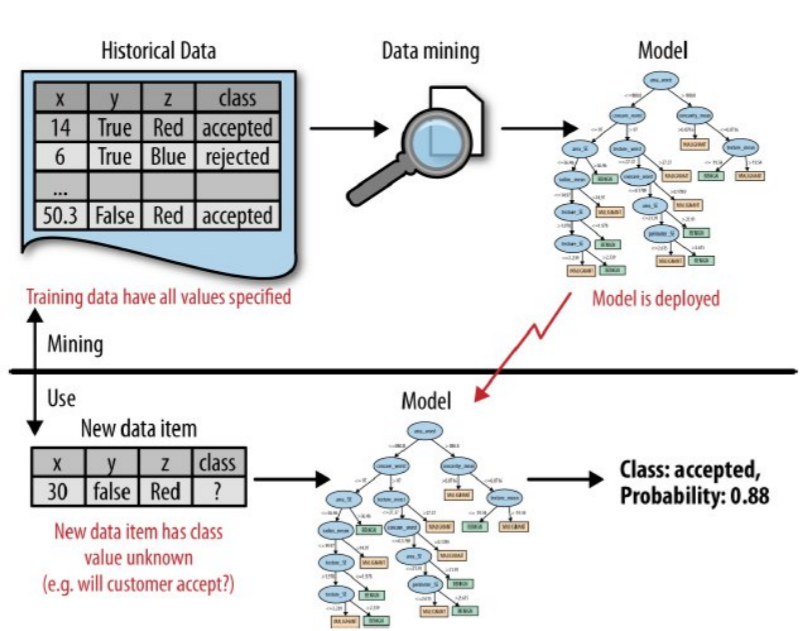
\includegraphics[width=0.6\textwidth]{images/Data_Mining.png}
    \caption{Data Mining}
    \label{fig:Data Mining}
\end{figure}

\noindent
\begin{minipage}[t]{0.45\textwidth}
    
        \vspace{1.5cm}
        Linear models represent functions with:
            \begin{compactitemize}
                \item \textbf{Inputs}: attribute values
                \item \textbf{Output}: sum of weighted attribute values
            \end{compactitemize}
        The model determines optimal weight values. In two dimensions, this creates a straight line through data points.
        
        \textbf{Example}: $PRP = 37.06 + 2.47 \cdot CACH$
        
\end{minipage}
\hfill
\begin{minipage}[t]{0.5\textwidth}
    \vspace{0.5cm} % Aggiusta lo spazio verticale per allineare meglio l'immagine
    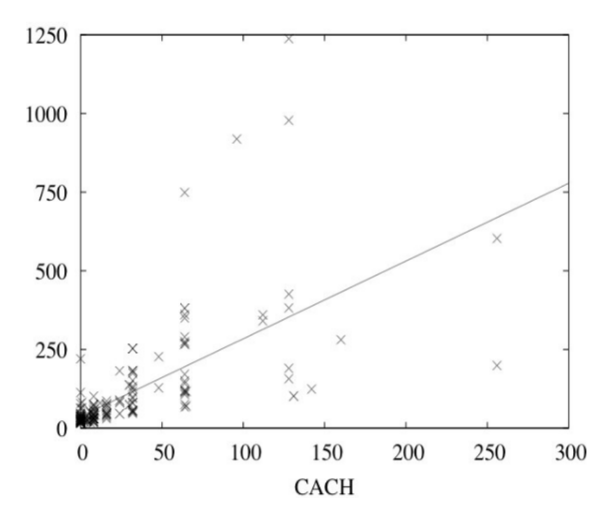
\includegraphics[width=\textwidth]{images/linear_function.png}
    \captionof{figure}{Linear Function}
    \label{fig:Linear_Function}
\end{minipage}

\newpage

    For binary classification tasks:
\begin{compactitemize}
    \item The line separates two classes
    \item \textbf{Decision boundary}: defines where classification changes from one class to another
    \item Prediction rule: predict one class if output $\geq 0$, other class if output $< 0$
\end{compactitemize}
With multiple attributes, the decision boundary becomes a high-dimensional hyperplane.



\begin{figure}[H]
    \centering
    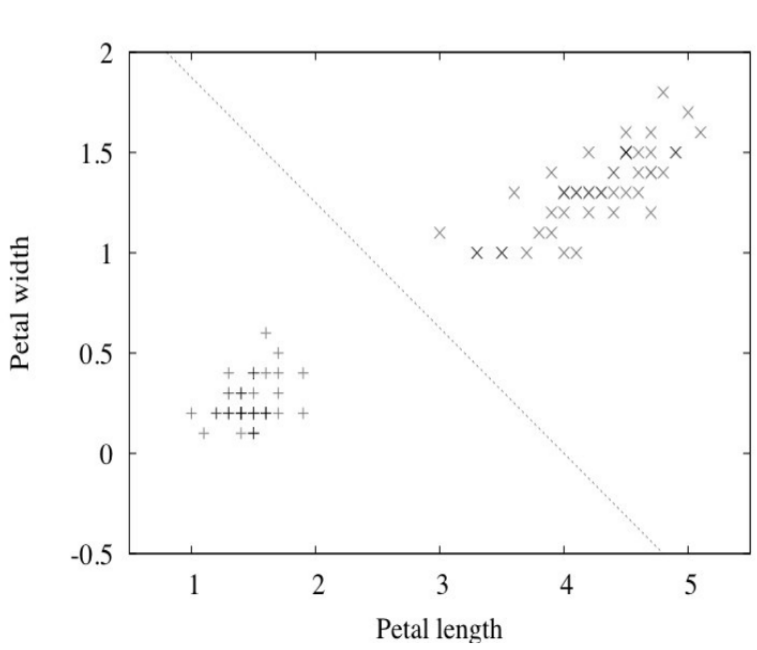
\includegraphics[width=0.3\textwidth]{images/binary_classification.png}
    \caption{Binary Classification}
    \label{fig:Binary Classification}
\end{figure}


\subsection{Decision Trees}

    Decision trees work with a "divide-and-conquer" approach. Each node in the tree tests a specific attribute, typically by comparing its value to a constant. The leaves of the tree assign a classification or probability distribution to instances. To make predictions, we route an unknown instance down the tree following the test results.

    When dealing with missing values, we need to consider whether the absence has significance. If it does, we treat "missing" as a separate value. If not, we split the instance into pieces weighted according to how training instances are distributed across branches.


\begin{figure}[H]
    \centering
    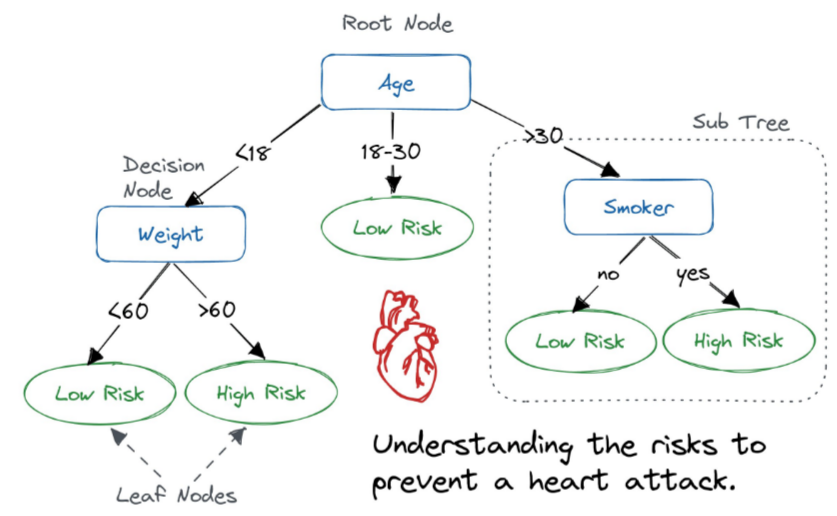
\includegraphics[width=0.6\textwidth]{images/Trees.png}
    \caption{Decision Trees}
    \label{fig:Decision Trees}
\end{figure}

\subsection{Classification Rules}

    Classification rules offer a popular alternative to decision trees. Each rule has an \textbf{antecedent} (the pre-condition with a series of tests) and a \textbf{consequent} (the conclusion assigning classes or probabilities). Rules are typically combined with logical OR operations, though this can create conflicts when different rules suggest different conclusions.

    Converting trees to rules is straightforward: create one rule for each leaf, where the antecedent contains conditions from the root to that leaf. This produces unambiguous rules that work regardless of execution order, but they're often unnecessarily complex and require pruning.


\subsection{Instance-Based Learning}

    Instance-based learning represents the simplest form of machine learning through rote memorization. The system stores all training instances and, when facing a new case, searches for the most similar stored instance. This approach is called "lazy learning" because the real work happens during prediction rather than training.

    For measuring similarity, we use distance functions. With numeric attributes, we typically use Euclidean distance after normalizing the data. For nominal attributes, the distance is 1 if values differ and 0 if they're equal. Often, we need to weight attributes differently based on their importance.


\section{Algorithms: The Basic Methods}

\subsection{Building a Decision Tree}

    To build a decision tree we'll use the top down staryegy. The main steps are:
    \begin{compactitemize}
        \item Decison which attribute we'll use to split the data at time $t$.
        \item Create the son nodes, obtained by splitting the data according to the attribute's values.
        \item Repeat the process recursively for each son node, until a stopping criterion is met.
    \end{compactitemize}

    If the professor had been a good memory, he would remebered to put the dataset example in the slides, but he didn't. So we'll continue without the image dataset example:


\begin{figure}[H]
    \centering
    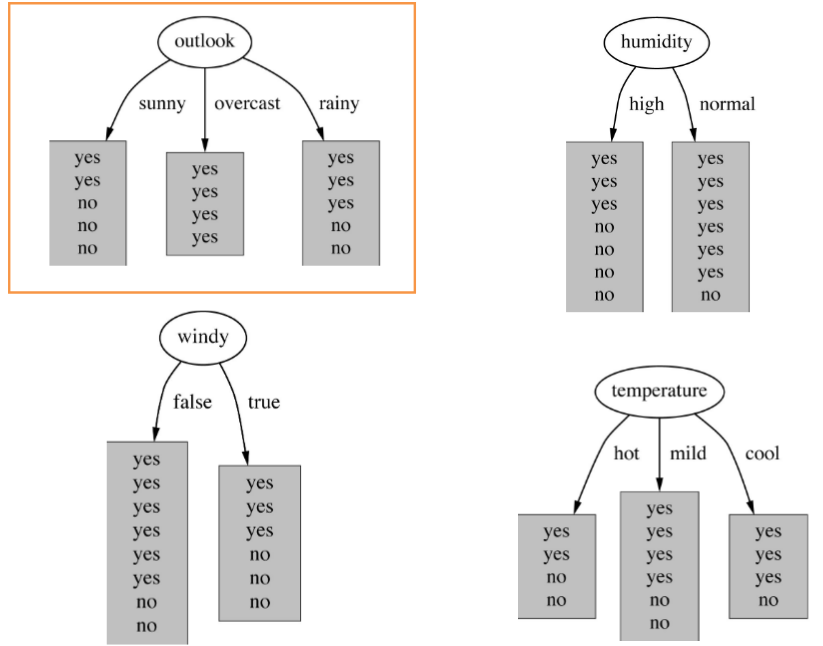
\includegraphics[width=0.6\textwidth]{images/Attribute_selection.png}
    \caption{Attribute Selection }
    \label{fig:Attribute Selection }
\end{figure}

\subsection{Criteria for Attribute Selection}

    When building decision trees, determining which attribute to use for splitting the data is crucial. Our primary objective is to construct the smallest possible tree, which leads us to adopt a heuristic approach: choosing the attribute that produces the "purest" nodes. The most popular purity criterion is \emph{information gain}, which increases with the average purity of the resulting subsets. Therefore, our strategy is to select the attribute that provides the greatest information gain at each step of the tree construction process.



\subsection{Entropy}

    The purity may be measured through the "information" needed to specify whether a new instance should be classified yes/no, given that the example reached the node.
    
    \begin{compactitemize}
        \item Information is measured in bits
        \item Entropy gives the information required in bits (can involve fractions of bits!)
        \item Formula for computing the entropy:
    \end{compactitemize}
    
    \begin{equation}
    entropy(p_1, p_2, ..., p_n) = -p_1\log p_1 - p_2\log p_2 - ... - p_n\log p_n
    \end{equation}


\subsection{Entropy of the Attribute Outlook}

    \textbf{Outlook = Sunny:}\\
    $info(2,3) = entropy(\frac{2}{5}, \frac{3}{5}) = -\frac{2}{5}\log(\frac{2}{5}) - \frac{3}{5}\log(\frac{3}{5}) = 0.971$ bits\\
    
    \textbf{Outlook = Overcast:}\\
    $info(4,0) = entropy(1,0) = -1\log(1) - 0\log(0) = 0$ bits\\
    
    \textbf{Outlook = Rainy:}\\
    $info(3,2) = entropy(\frac{3}{5}, \frac{2}{5}) = -\frac{2}{5}\log(\frac{2}{5}) - \frac{3}{5}\log(\frac{3}{5}) = 0.971$ bits\\
    
    \textbf{Expected information for attribute:}\\
    $info(2,3; 4,0; 3,2) = (\frac{5}{14}) \times 0.971 + (\frac{4}{14}) \times 0 + (\frac{5}{14}) \times 0.971 = 0.693$ bits


\subsection{Computing Information Gain}

    \textbf{Information gain:} information before splitting – information after splitting\\
    
    \begin{equation}
    gain(Attribute) = info(before) - info(after)
    \end{equation}
    
    Information gain for attributes from weather data:
    \begin{compactitemize}
        \item $gain(Outlook) = info([9,5]) - info([2,3],[4,0],[3,2]) = 0.940 - 0.693 = 0.247$ bits
        \item $gain(Outlook) = 0.247$ bits
        \item $gain(Temperature) = 0.029$ bits  
        \item $gain(Humidity) = 0.152$ bits
        \item $gain(Windy) = 0.048$ bits
    \end{compactitemize}



    To obtain the final decision tree, we repeat the process recursively for each son node, until a stopping criterion is met. The stopping criteria can be, ad example, when all instances at a node belong to the same class, or when there are no remaining attributes to split on. 



\begin{figure}[H]
    \centering
    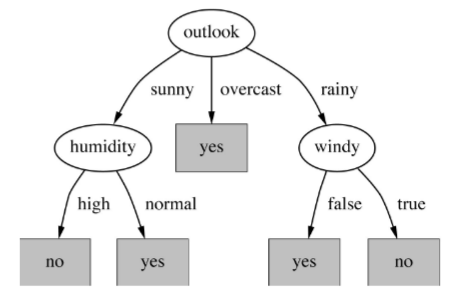
\includegraphics[width=0.6\textwidth]{images/final_tree.png}
    \caption{Final Decision Tree }
    \label{fig:Final Decision Tree }
\end{figure}


\subsection{Highly-branching Attributes}

    Attributes with a large number of values can be problematic in decision tree construction. In the extreme case, consider an ID code attribute where each instance has a unique value. Such subsets are more likely to be pure simply because there is a large number of possible values, making information gain biased towards choosing attributes with many values. This bias may result in overfitting, leading to the selection of attributes that are non-optimal for prediction.
    
    For example, the entropy of split for ID code would be:
    \begin{equation}
        info_{ID\ code} = info(0,1) + info(0,1) + ... + info(0,1) = 0\ bits
    \end{equation}
    
    
    This makes information gain maximal for ID code (namely 0.940 bits), even though it provides no meaningful predictive power.



\begin{figure}[H]
    \centering
    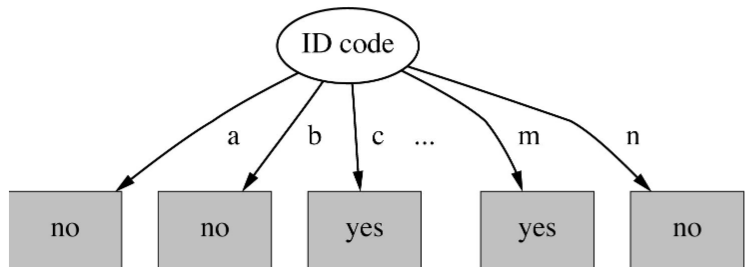
\includegraphics[width=0.6\textwidth]{images/id_code.png}
    \caption{Final ID code examples }
    \label{fig:ID code examples }
\end{figure}


\subsection{Gain Ratio}

    The gain ratio is a modification of information gain that reduces its bias towards attributes with many values. It takes both the number and size of branches into account when choosing an attribute, correcting information gain by considering the intrinsic information of a split.
    
    \textbf{Intrinsic information} represents the entropy of distribution of instances into branches - essentially, how much information we need to tell which branch an instance belongs to.
    
    \begin{equation}
    gain\_ratio(attribute) = \frac{gain(attribute)}{intrinsic\_info(attribute)}
    \end{equation}
    
    Example for ID code:
    $info(1,1,...,1) = 14 \times (-\frac{1}{14} \times \log\frac{1}{14}) = 3.807\ bits$
    $gain\_ratio(ID\ code) = \frac{0.940\ bits}{3.807\ bits} = 0.246$
    
    The value of the attribute decreases as intrinsic information gets larger, effectively penalizing attributes with many branches.


\newpage
\subsection{Gain Ratios for Weather Data}

    Calculating gain ratios for all attributes in the weather data:
    
    \begin{center}
    \begin{tabular}{|c|c|c|c|c|}
    \hline
    \textbf{Attribute} & \textbf{Info} & \textbf{Gain} & \textbf{Split Info} & \textbf{Gain Ratio} \\
    \hline
    Outlook & 0.693 & 0.247 & info([5,4,5]) = 1.577 & 0.247/1.577 = 0.157 \\
    Temperature & 0.911 & 0.029 & info([4,6,4]) = 1.557 & 0.029/1.557 = 0.019 \\
    Humidity & 0.788 & 0.152 & info([7,7]) = 1.000 & 0.152/1 = 0.152 \\
    Windy & 0.892 & 0.048 & info([8,6]) = 0.985 & 0.048/0.985 = 0.049 \\
    \hline
    \end{tabular}
    \end{center}


\subsection{More on the Gain Ratio}

    While "Outlook" still comes out as the top choice, the ID code would have an even greater gain ratio in this scenario. The standard fix is to implement an ad hoc test to prevent splitting on attributes of this type.
    
    However, gain ratio has its own problem: it may overcompensate by choosing an attribute simply because its intrinsic information is very low. The standard solution is to only consider attributes with greater than average information gain, ensuring that we don't select attributes with artificially inflated ratios due to very small intrinsic information values.


\subsection{Regression via mathematical functions}

    In linear regression, the linear function estimates the numeric target value while the training data provide the actual target value. An intuitive notion of model fit is measuring how far away the estimated values are from the true values on the training data - in other words, how big is the error of the fitted model? We would like to minimize this error.
    
    \begin{equation}
    x = w_0 + w_1 a_1 + w_2 a_2 + ... + w_k a_k
    \end{equation}
    
    For a particular training dataset, we can compute this error for each individual data point and sum up the results. The model that fits the data best would be the model with the minimum sum of errors on the training data.


\subsection{Error Computation Methods}

    There are many ways to compute the error between an estimated and an actual value. One approach is the absolute error: subtracting one from the other and taking the absolute value. However, standard linear regression uses the squares of these errors.
    
    Why do people use least squares regression without much thought to alternatives? It strongly penalizes very large errors. One might ask: why not take the fourth power of the errors and penalize large errors even more strongly? Importantly, any choice for the objective function has both advantages and drawbacks.
    
    For least squares regression, a serious drawback is that it is very sensitive to the data: erroneous or outlying data points can severely skew the resultant linear function.


\subsection{Weight Calculation in Linear Regression}

    Weights are calculated from the training data. The predicted value for the first training instance $a^{(1)}$ (assuming each instance is extended with a constant attribute with value 1) is:
    
    \begin{equation}
    w_0a_0^{(1)} + w_1a_1^{(1)} + w_2a_2^{(1)} + ... + w_ka_k^{(1)} = \sum_{j=0}^{k} w_ja_j^{(1)}
    \end{equation}
    
    We choose $k+1$ coefficients to minimize the squared error on the training data. The squared error to be minimized is:
    
    \begin{equation}
    \sum_{i=1}^{n} \left(x^{(i)} - \sum_{j=0}^{k} w_ja_j^{(i)}\right)^2
    \end{equation}
    
    This formulation allows us to find the optimal weights that minimize the total squared error across all training instances.


\subsection{Class Probability Estimation and Logistic ``Regression''}

    By choosing a different objective function, we can produce a model designed to give accurate estimates of class probability rather than just predicting class membership. The most common procedure for this purpose is logistic regression.
    
    One useful notion of the likelihood of an event is the odds. The odds of an event is the ratio of the probability of the event occurring to the probability of the event not occurring. If we cared about modeling some notion of likelihood, rather than the class membership probability specifically, we could model the log-odds with $f(x)$.
    
    \begin{equation}
        f(x) = w_0 + w_1 a_1 + w_2 a_2 + \ldots + w_k a_k
    \end{equation}
    
    This is exactly a logistic regression model: the same linear function $f(x)$ is used as a measure of the log-odds of the ``event'' of interest. Here, $f(x)$ is the model's estimation of the log-odds that $x$ belongs to the positive class. For example, the model might estimate the log-odds that a customer described by feature vector $x$ will leave the company when her contract expires.


\subsection{Logistic Regression: Technical Details}
    In logistic regression, $p^+(x)$ represents the model's estimate of the probability of class membership of a data item represented by feature vector $x$. The class $+$ is whatever binary event we are modeling, and the estimated probability of the event not occurring is therefore $(1 - p^+(x))$.
    
    The fundamental relationship in logistic regression specifies that for a particular data item described by feature vector $x$, the log-odds of the class is equal to our linear function $f(x)$:
    
    \begin{equation}
        \log\left(\frac{p^+(x)}{1 - p^+(x)}\right) = f(x)
    \end{equation}
    
    Since we often want the estimated probability of class membership rather than the log-odds, we can solve for $p^+(x)$ by applying the logistic function, which transforms the linear output into a probability between 0 and 1.
    The logistic function is defined as:
    \begin{equation}
        p^+(x) = \frac{1}{1 + e^{-f(x)}}
    \end{equation}

\subsection{Instance-Based Learning}
For measuring similarity, we use distance functions. With numeric attributes, we typically use Euclidean distance after normalizing the data. For nominal attributes, the distance is 1 if values differ and 0 if they're equal. Often, we need to weight attributes differently based on their importance.

    Training examples are stored in memory, and the distance function defines what's learned. Most instance-based schemes use Euclidean distance to measure similarity between instances. Given two instances $a^{(1)}$ and $a^{(2)}$ with $k$ attributes, the Euclidean distance is calculated as:

    \begin{equation}
    distance(a^{(1)}, a^{(2)}) = \sqrt{(a_1^{(1)} - a_1^{(2)})^2 + (a_2^{(1)} - a_2^{(2)})^2 + ... + (a_k^{(1)} - a_k^{(2)})^2}
    \end{equation}

    Note that taking the square root is not required when comparing distances, as the ordering remains the same. Another popular metric is the city-block (Manhattan) metric, which sums the absolute differences instead of squared differences.
   
    \textbf{Note:} We take the squared differences because we want to penalize large differences more than small ones. For example, a difference of 2 should be penalized more than twice a difference of 1.

\subsection{Normalization}

    Different attributes are often measured on different scales, which can cause problems when computing distances. Therefore, attributes need to be normalized to ensure fair comparison. For numeric attributes, we use the following normalization formula:

    \begin{equation}
    a_i = \frac{v_i - \min v_i}{\max v_i - \min v_i}
    \end{equation}

    where $v_i$ is the actual value of attribute $i$, and $\min v_i$ and $\max v_i$ are the minimum and maximum values of that attribute in the dataset, respectively. This normalization scales all numeric attributes to the range $[0,1]$.

    For nominal attributes, the distance is either 0 (if values are equal) or 1 (if values differ). 

    The usual policy for missing values is to assume they are maximally distant from all other values, which translates to a distance of 1 for normalized attributes.


    \subsection{k-Nearest Neighbors (k-NN)}
    The k-Nearest Neighbors algorithm is a fundamental instance-based learning method used for both classification and regression tasks. The basic procedure is straightforward:
    \begin{compactitemize}
        \item Given a new example whose target variable we want to predict, we scan through all the training examples.
        \item We select several examples that are most similar to the new example (the "nearest neighbors").
        \item We predict the new example's target value based on the nearest neighbors' known target values using a combining function.
    \end{compactitemize}
    
    The combining function can be voting (for classification) or averaging (for regression), operating on the neighbors' known target values to produce a prediction.
    
    \subsubsection{k-NN for Classification}
    
    For classification tasks, the process works as follows:
    \begin{compactitemize}
        \item The label we want to predict is indicated by a "?".
        \item The k nearest neighbors are retrieved and their known target variables (classes) are consulted.
        \item A simple combining function is majority vote: the class that appears most frequently among the k neighbors is assigned to the new instance.
    \end{compactitemize}
    
    For example, if we use 3-NN and retrieve three neighbors where two are positive and one is negative, majority voting would predict the positive class.
    
    \textbf{Probability Estimation:} Beyond simple classification, it's usually important to estimate the probability of class membership. k-NN can do this easily by computing the proportion of neighbors belonging to each class. In the example above, the probability of the positive class would be estimated as $\frac{2}{3}$.
    
    \subsubsection{Choosing k and Weighting Neighbors}
    
    \textbf{How many neighbors should be used?}
    \begin{compactitemize}
        \item Odd numbers are convenient for breaking ties in majority vote classification with two-class problems.
        \item Nearest neighbor algorithms are referred to as k-NN, where k refers to the number of neighbors used (e.g., 3-NN).
        \item The greater k is, the more the estimates are smoothed out among neighbors.
        \item If we increase k to the maximum possible (k = n, the entire dataset), we would predict the average over the entire dataset for any example:
        \begin{compactitemize}
            \item For classification: predicting the majority class in the entire dataset.
            \item For regression: predicting the average of all target values.
        \end{compactitemize}
    \end{compactitemize}
    
    \textbf{Should we treat all neighbors the same?}
    
    Different neighbors have different similarity to the example we're trying to predict, which should influence how they're used. The simple majority voting strategy ignores how close each neighbor is to the instance.
    
    Nearest-neighbor methods often use \textbf{weighted voting} or \textbf{similarity-moderated voting}, where each neighbor's contribution is scaled by its similarity to the query instance. A common approach is using the reciprocal of the square of the distance as the scaling weight:
    
    \begin{equation}
    weight_i = \frac{1}{distance(x, x_i)^2}
    \end{equation}
    
    This ensures that closer neighbors have more influence on the prediction than distant ones.
    
    \subsubsection{Geometric Interpretation and Overfitting}
    
    Although k-NN does not create an explicit decision boundary during training, there are implicit regions created by instance neighborhoods. These regions can be calculated by systematically probing points in the instance space, determining each point's classification, and constructing the boundary where classifications change.
    
    \textbf{Overfitting and Complexity Control:}
    
    The parameter k in a k-NN classifier acts as a complexity parameter that controls overfitting:
    \begin{compactitemize}
        \item \textbf{At one extreme (k = n):} We do not allow much complexity at all in our model. The n-NN model simply predicts the average value in the dataset for each case, resulting in an extremely simple model.
        \item \textbf{At the other extreme (k = 1):} We get an extremely complex model that places complicated boundaries such that every training example will be in a region labeled by its own class. The 1-NN classifier is prone to overfitting, as it can be heavily influenced by outliers and noise in the training data.
        \item \textbf{Intermediate values of k:} Provide a balance between model complexity and generalization ability.
    \end{compactitemize}
    
    \textbf{How should one choose k?}
    
    The optimal value of k should be determined through experimental evaluation, typically using cross-validation on the training data to find the value that provides the best balance between bias and variance.


    \begin{figure}[H]
        \centering
        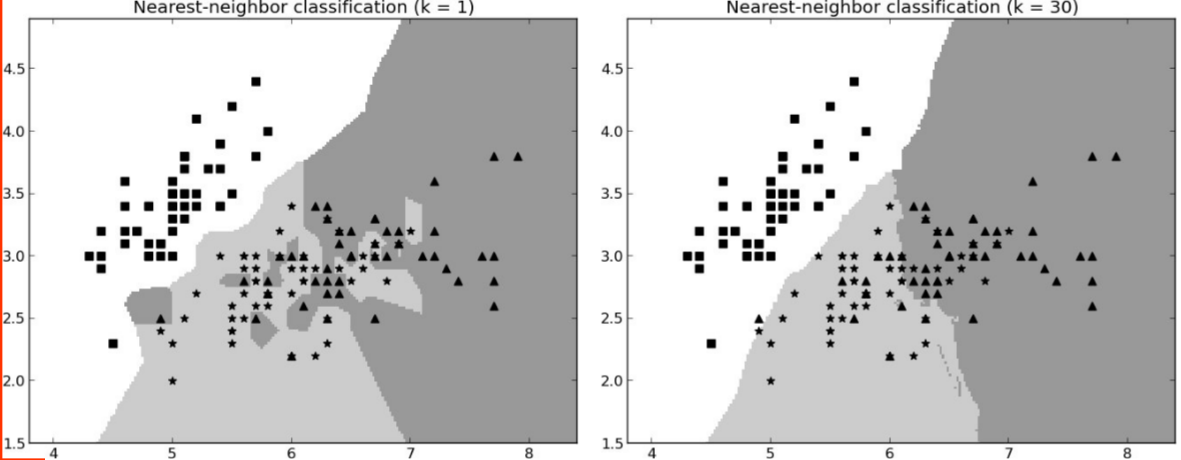
\includegraphics[width=0.8\textwidth]{images/KKN.png}
        \caption{Differences between 1-NN and 30-NN }
        \label{fig:Difference_between_1-NN_and_30-NN }
    \end{figure}

    \begin{figure}[H]
        \centering
        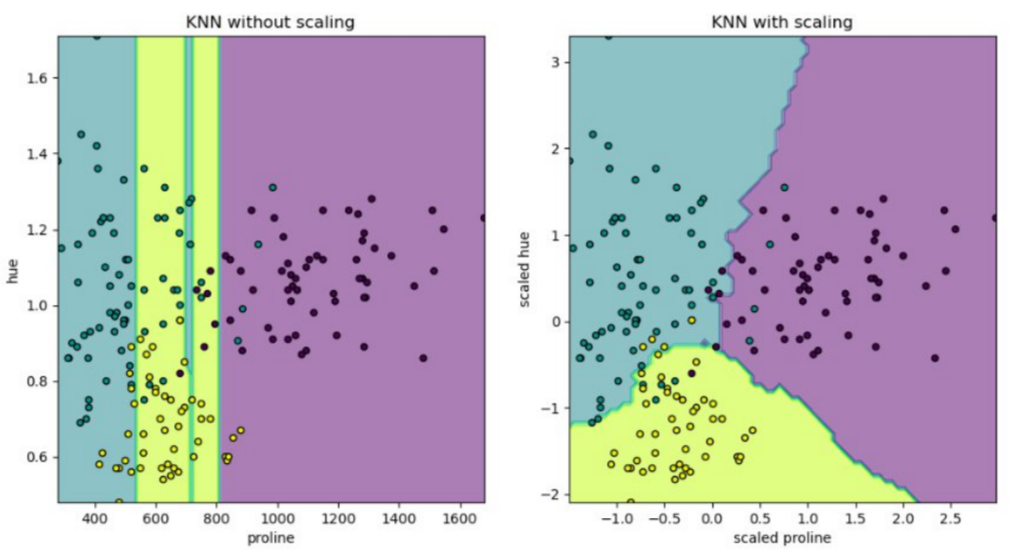
\includegraphics[width=0.9\textwidth]{images/scaler.png}
        \caption{Important of the standard scaler }
        \label{fig:Important_of_the_standard_scaler }
    \end{figure}


    \subsection{Clustering Techniques}

    Clustering techniques are traditionally divided into two main categories: partitioning and hierarchical algorithms.
    
    \textbf{Partitioning algorithms} construct a partition of a database $D$ of $n$ objects into a set of $k$ clusters, where $k$ is an input parameter. The algorithm starts with an initial partition and uses an iterative strategy to optimize an objective function. Each cluster is typically represented by its centroid (gravity center).
    
    The procedure consists of two steps:
    \begin{compactitemize}
        \item Determine $k$ representatives that minimize the objective function
        \item Assign each object to the cluster with the closest representative
    \end{compactitemize}
    
    \textbf{Hierarchical algorithms} create a hierarchical decomposition of $D$ represented by a dendrogram (a tree structure). The dendrogram iteratively splits $D$ into smaller subsets until each subset consists of a single object. Each node in the tree represents a cluster. The dendrogram can be created:
    \begin{compactitemize}
        \item \textbf{Bottom-up} (agglomerative): from leaves to root by merging clusters
        \item \textbf{Top-down} (divisive): from root to leaves by dividing clusters
    \end{compactitemize}
    
    Unlike partitioning algorithms, hierarchical methods do not require $k$ as input.
    
    \subsubsection{Data Representation and Distance Metrics}
    
    A clustering dataset is a collection of points belonging to some space. In Euclidean spaces:
    \begin{compactitemize}
        \item Points are vectors of real numbers
        \item Vector length = number of dimensions
        \item Vector components = coordinates of points
        \item Euclidean distance is the standard metric: $\sqrt{\sum_{i=1}^{d}(x_i - y_i)^2}$
    \end{compactitemize}
    
    For non-Euclidean spaces, alternative distance measures include Jaccard distance, cosine distance, and Hamming distance.
    
    \subsubsection{Hierarchical Clustering Algorithm}
    
    The general procedure for hierarchical clustering:
    \begin{enumerate}
        \item Start with each point in its own cluster
        \item Iteratively combine the two nearest clusters
        \item Continue until a stopping criterion is met
    \end{enumerate}
    
    Three key design decisions must be made:
    
    \textbf{1. Cluster Representation:} For Euclidean spaces, we typically use the centroid (average of all points in the cluster).
    
    \textbf{2. Inter-cluster Distance:} We measure distance between clusters using their centroids (though other methods exist, such as single-linkage or complete-linkage).
    
    \textbf{3. Stopping Criteria:}
    \begin{compactitemize}
        \item Stop at a predetermined number of clusters (if known a priori)
        \item Stop when cluster quality falls below a threshold
        \item Build the complete dendrogram and let the user choose the cut level
    \end{compactitemize}
    
    \subsubsection{K-Means Algorithm}
    
    K-means is a popular partitioning algorithm that works as follows:
    
    \textbf{Algorithm:}
    \begin{enumerate}
        \item \textbf{Initialization:} Select $k$ initial points as cluster centers
        \item \textbf{Assignment:} Assign each remaining point to the nearest centroid
        \item \textbf{Update:} Recalculate centroids as the mean of assigned points
        \item \textbf{Iterate:} Repeat steps 2-3 until convergence
        \item \textbf{Refinement (optional):} Reassign all points to final centroids
    \end{enumerate}
    
    The centroid of a cluster can migrate as points are assigned, but since only nearby points are typically assigned, the centroid tends not to move dramatically between iterations.
    
    \subsection{Density-Based Clustering}
    
    Density-based methods identify clusters as dense regions separated by sparse areas. They can detect arbitrary-shaped clusters and automatically identify noise points.
    
    \subsubsection{DBSCAN Algorithm}
    
    DBSCAN (Density-Based Spatial Clustering of Applications with Noise) uses two parameters:
    \begin{compactitemize}
        \item $\epsilon$ (Eps): maximum distance between neighbors
        \item MinPts: minimum points to form a dense region
    \end{compactitemize}
    
    \textbf{Core Concepts:}
    \begin{compactitemize}
        \item \textbf{Core points:} points with at least MinPts neighbors within $\epsilon$
        \item \textbf{Border points:} non-core points within $\epsilon$ of a core point
        \item \textbf{Noise points:} points that are neither core nor border points
    \end{compactitemize}

    \begin{figure}[H]
        \centering
        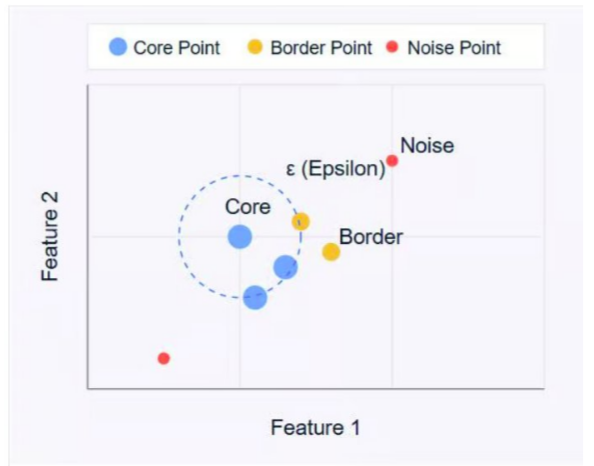
\includegraphics[width=0.5\textwidth]{images/Point.png}
        \caption{Point for DBSCAN }
        \label{fig:Point_for_DBSCAN }
    \end{figure}

    
    \textbf{Formal Definitions:}
    
    \textbf{Definition 1 (Eps-neighborhood):}
    \begin{equation}
    N_{Eps}(p) = \{q \in D \mid dist(p, q) \leq Eps\}
    \end{equation}
    
    \textbf{Definition 2 (Directly density-reachable):} Point $p$ is directly density-reachable from $q$ if:
    \begin{compactitemize}
        \item $p \in N_{Eps}(q)$, and
        \item $|N_{Eps}(q)| \geq MinPts$ (core point condition)
    \end{compactitemize}
    
    Note: This relation is symmetric for core point pairs, but asymmetric for core-border pairs.


    \begin{figure}[H]
        \centering
        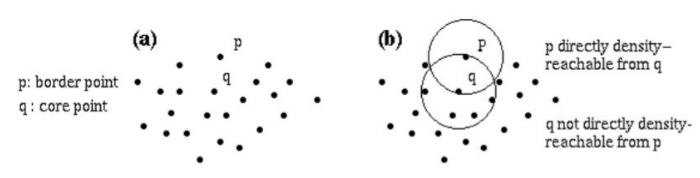
\includegraphics[width=0.7\textwidth]{images/Def_1_2.png}
        \caption{Definitions 1 and 2 for DBSCAN }
        \label{fig:Definitions_1_and_2_for_DBSCAN }
    \end{figure}
    
    \textbf{Definition 3 (Density-reachable):} Point $p$ is density-reachable from $q$ if there exists a chain $p_1 \rightarrow p_2 \rightarrow \ldots \rightarrow p_n$ where $p_1 = q$, $p_n = p$, and each $p_{i+1}$ is directly density-reachable from $p_i$. This relation is transitive but not symmetric.
    
    \textbf{Definition 4 (Density-connected):} Points $p$ and $q$ are density-connected if both are density-reachable from some point $o$. This relation is symmetric.
    
    \begin{figure}[H]
        \centering
        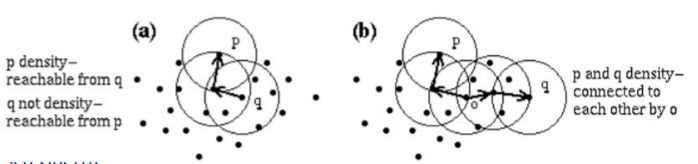
\includegraphics[width=0.7\textwidth]{images/Def_3_4.png}
        \caption{Definitions 3 and 4 for DBSCAN }
        \label{fig:Definitions_3_and_4_for_DBSCAN }
    \end{figure}
    

    \textbf{Definition 5 (Cluster):} A cluster $C$ is a maximal set of density-connected points:
    \begin{compactitemize}
        \item \textbf{Maximality:} If $p \in C$ and $q$ is density-reachable from $p$, then $q \in C$
        \item \textbf{Connectivity:} All points in $C$ are mutually density-connected
    \end{compactitemize}
    
    \textbf{Definition 6 (Noise):} Points not belonging to any cluster: $noise = \{p \in D \mid \forall i: p \notin C_i\}$

    
    \textbf{DBSCAN Procedure:}
    \begin{enumerate}
        \item Choose parameters $\epsilon$ and MinPts
        \item Select an arbitrary unvisited point
        \item Find all points within $\epsilon$ distance
        \item If fewer than MinPts neighbors: mark as noise (temporarily)
        \item If at least MinPts neighbors: create new cluster with this core point
        \item Recursively add all density-reachable points to the cluster
        \item Repeat from step 2 until all points are visited
        \item Finalize: noise points near clusters become border points
    \end{enumerate}
    
    \subsubsection{HDBSCAN Algorithm}
    
    HDBSCAN (Hierarchical DBSCAN) extends DBSCAN by:
    \begin{compactitemize}
        \item Building a cluster hierarchy for all density levels
        \item Extracting stable clusters using a stability measure
        \item Not requiring a global $\epsilon$ parameter
    \end{compactitemize}
    
    \textbf{Mutual Reachability Distance:}
    
    The core distance of point $x$ is the distance to its MinPts-th nearest neighbor:
    \begin{equation}
    d_{core}(x) = \text{distance to MinPts-th nearest neighbor}
    \end{equation}
    
    The mutual reachability distance between points $x_p$ and $x_q$ is:
    \begin{equation}
    MRD(x_p, x_q) = \max\{d_{core}(x_p), d_{core}(x_q), d(x_p, x_q)\}
    \end{equation}
    
    This metric improves robustness by ensuring sparse points (potential noise) maintain at least their core distance from others.
    
    \textbf{Algorithm Steps:}
    
    \textbf{1. Build Hierarchy:}
    \begin{compactitemize}
        \item Construct a graph with points as nodes and MRD as edge weights
        \item Build a Minimum Spanning Tree (MST)
        \item Sort edges by MRD to create a dendrogram
    \end{compactitemize}
    
    \textbf{2. Condense Tree:} Simplify the hierarchy by pruning:
    \begin{compactitemize}
        \item Both children have $\geq$ MinPts $\rightarrow$ valid split
        \item Both children have $<$ MinPts $\rightarrow$ cluster disappears
        \item One child has $<$ MinPts $\rightarrow$ child becomes noise, parent continues
    \end{compactitemize}
    
    \textbf{3. Select Clusters:}
    \begin{compactitemize}
        \item \textbf{Simple approach:} Select all leaf nodes (fine-grained clustering)
        \item \textbf{EOM (Excess of Mass):} Select clusters that maximize total stability across the partition
    \end{compactitemize}
    
    Stability measures how consistently a cluster exists across density levels—stable clusters form early, persist long, and retain many points.
    
    \subsection{Clustering Performance Evaluation}
    
    \subsubsection{Adjusted Rand Index}
    
    Measures similarity between two partitions (e.g., predicted vs. ground truth):
    \begin{compactitemize}
        \item Counts agreement on all pairs of points
        \item Same cluster in both partitions $\rightarrow$ agreement
        \item Different clusters in both $\rightarrow$ agreement
        \item Otherwise $\rightarrow$ disagreement
    \end{compactitemize}
    
    Values: 1 = perfect match, 0 = random labeling, $< 0$ = worse than random. The adjustment corrects for chance agreement.
    
    \subsubsection{Silhouette Coefficient}
    
    Internal validation metric (no ground truth needed). For each point $i$:
    \begin{compactitemize}
        \item $a(i)$ = average distance to points in same cluster (cohesion)
        \item $b(i)$ = minimum average distance to points in other clusters (separation)
    \end{compactitemize}
    
    Silhouette coefficient:
    \begin{equation}
    s(i) = \frac{b(i) - a(i)}{\max\{a(i), b(i)\}}
    \end{equation}
    
    Range: $[-1, 1]$. High values indicate dense, well-separated clusters. Models with high average silhouette coefficients cluster similar samples together and keep dissimilar samples apart.



\section{Data Preparation}